\chapter{Theoretische Grundlage}
\begin{wrapfigure}[26]{R}[34pt]{0.6\textwidth}

  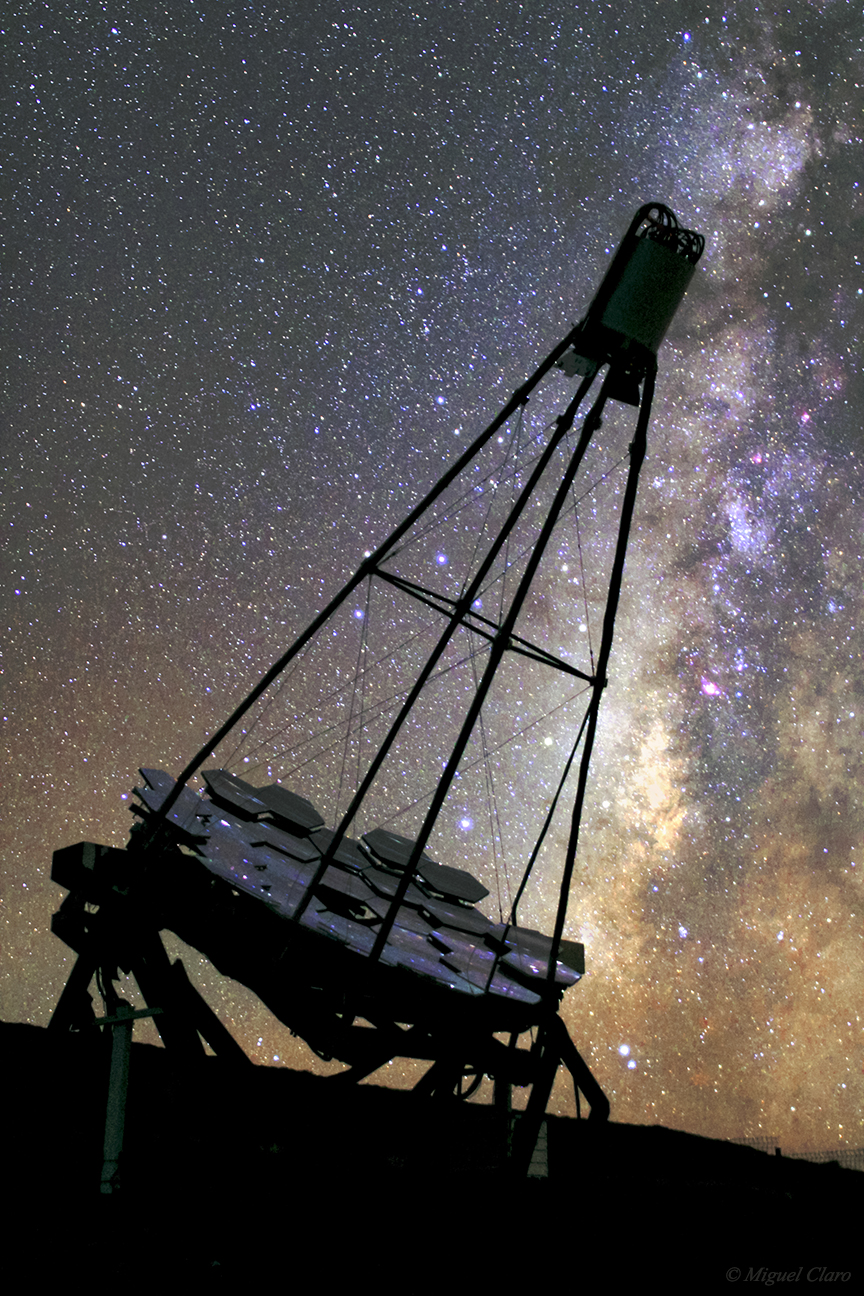
\includegraphics[width=0.5\textwidth]{./logos/FACT.jpg}
  \caption{FACT in Observatiosposition}
  \label{fig:observ}

\end{wrapfigure}
Für die statistische Sicherheit sind große Zählergebnisse von Vorteil. Um große Zählergebnisse zu erreichen besteht die möglichkeit die Observationszeit zu Maximieren. Dies wird getestet in dem das FACT (First G-APD Cherenkov Telescope) Teleskope aufgrund seiner Silzium Photomultiplier auch an Tagen mit starker diffuser Nacht-Hintergrundstrahlung aufgrund der neuartigen Technick der SiMPs betrieben werden kann. Das Cherenkov Teleskop befindet sich auf der kanarischen Insel Las Palma und dient momentan der Überwachung von starken Gammastrahlungsquellen um bei erhöhter Aktivität größere Teleskope zu informierern. \\
Das Projekt entstand als ein Nachfolgerexperiment des übergebliebenen HEGRA Telskope, wobei die übergeblieben Spiegel aufbereitet und wiederverwertet werden. Die 30 hexongonalen Spiegel bilden eine Gesamtspiegelfläche von \SI{9.51}{\meter\squared} bei einem Blickfeld von \SI{4.5}{\degree}. Dabei wird bei dem Tekeskop zum ersten mal Silizium Photomultiplier (SiPMs) verwendet anstelle von herkömlichen Photomultiplier Tubes. Halbleiterdetektoren lassen sich mit einer geringerren operation Spannung (< \SI{100}{\volt}) betreiben und sind preiswerter als Photomultiplier, was die Gestaltung des Kameradesigns, als auch die Finanzierung vereinfacht.
Dabei bilden 1440 Kamerapixel das Bild der Kamera, welche jeweils aus einem quadratischen Sensor und einem Plexiglasleiter bestehen. Die einzelne Oberflächen der Hexagonal zulaufenden Plexiglasleiter bilden dabei das Kamerabild.
